\documentclass[a4paper]{article}
\usepackage[utf8]{inputenc}
\usepackage[spanish, es-tabla, es-noshorthands]{babel}
\usepackage[table,xcdraw]{xcolor}
\usepackage[a4paper, footnotesep = 1cm, width=20cm, top=2.5cm, height=25cm, textwidth=18cm, textheight=25cm]{geometry}
%\geometry{showframe}

\usepackage{tikz}
\usepackage{amsmath}
\usepackage{amsfonts}
\usepackage{amssymb}
\usepackage{float}
\usepackage{graphicx}
\usepackage{caption}
\usepackage{subcaption}
\usepackage{multicol}
\usepackage{multirow}
\setlength{\doublerulesep}{\arrayrulewidth}
\usepackage{booktabs}

\usepackage{hyperref}
\hypersetup{
    colorlinks=true,
    linkcolor=blue,
    filecolor=magenta,      
    urlcolor=blue,
    citecolor=blue,    
}

\newcommand{\quotes}[1]{``#1''}
\usepackage{array}
\newcolumntype{C}[1]{>{\centering\let\newline\\\arraybackslash\hspace{0pt}}m{#1}}
\usepackage[american]{circuitikz}
\usetikzlibrary{calc}
\usepackage{fancyhdr}
\usepackage{units} 

\graphicspath{{../Ejercicio-1/}{../Ejercicio-2/}{../Ejercicio-3/}{../Ejercicio-4/}}

\pagestyle{fancy}
\fancyhf{}
\lhead{22.01 Teoría de Circuitos}
\rhead{Mechoulam, Lambertucci, Rodriguez Turco, Londero, Galdeman}
\rfoot{\centering \thepage}

\begin{document}

\subsection{Celda universal}
Las celdas universales es un conjunto de filtros RC activos de segundo orden, compuestos por amplificadores operacionales configurados de forma sumadora, restadora, integradora, amplificadora o atenuadora, puestos en cascada. Estas son también conocidas como celdas de variables de estado, debido al uso de dicho método para la resolución de las ecuaciones diferenciales. Este tipo de celdas se caracteriza por poseer bajas sensibilidades con respecto a sus componentes, alta flexibilidad y buen rendimiento. Existen distintos tipos de configuraciones, donde cada una de estas posee sus respectivas ventajas y desventajas. A continuación, se procede a analizar cada una de ellas\footnote{L. Huelsman, Active and passive analog filter design, 2nd ed. New York: McGraw-Hill, 1993.}\footnote{R. Raut and M. N. S. Swamy, Modern Analog Filter Analysis and Design, 1st. ed. Weinheim: John Wiley and Sons, 2010.}.

\subsubsection{Kerwin-Huelsman-Newcomb (KHN)}
La celda Kerwin-Huelsman-Newcomb, nombre otorgado a partir de sus creadores\footnote{W. J. Kerwin, L. P. Huelsman and R. W. Newcomn, ``State-Variable Synthesis for Insensitive Integrated Circuit Transfer Functions  IEEE Journals \& Magazine'', Ieeexplore.ieee.org, 2019. [Online]. Available: \url{https://ieeexplore.ieee.org/document/1049798}. [Accessed: 20- Oct- 2019].}, puede ser comprendida con mayor facilidad a partir de un ejemplo. Se considera una transferencia de un filtro pasa banda:
\begin{equation}
	\frac{V_o(s)}{V_i(s)} = \frac{Ks}{s^2 + a_1 s + a_0}
\end{equation}

Se divide, tanto el numerador como el denominador de la expresión de la izquierda, por $s^2$.
\begin{equation}
	\frac{V_o(s)}{V_i(s)} = \frac{\frac{K}{s}}{1 + \frac{a_1}{s} + \frac{a_0}{s^2}}
	\label{equ:1}
\end{equation}

Siendo
\begin{equation}
	V_a(s) = frac{V_i(s)}{1 + \frac{a_1}{s} + \frac{a_0}{s^2}}
	\label{equ:2}
\end{equation}

Reescribinedo (\ref{equ:1}), se obtiene
\begin{equation}
	V_o(s) = \frac{K}{s} \cdot V_a(s)
	\label{equ:3}
\end{equation}

Si se utiliza la transformada de Laplace inversa tanto en (\ref{equ:2}) como en (\ref{equ:3}), se observa que se posee
\begin{equation}
\begin{split}
	v_a(t) =\ v_i(t) - a_1 & \int v_a(t)dt - a_0 \int \left( \int v_a(t)dt \right) dt \\
	v_o(t) =& \ K\int \left( \int v_a(t)dt \right) dt
\end{split}
\end{equation}

Del sistema anterior, $v_a(t) = \ddot{x}(t) $, $\int v_a(t)dt = \dot{x}(t)$ y $\int \left( \int v_a(t)dt = x(t) \right) dt$ son las llamadas variables de estado. Es más fácil de interpretar estas observando la Figura (\ref{fig:block}).

\begin{figure}[H]
\centering
	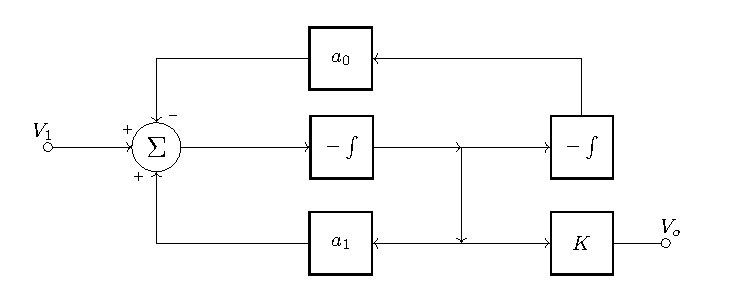
\includegraphics[width=0.7\textwidth]{ImagenesEjercicio4/Diagrama-De-Bloques.pdf}
	\caption{Diagrama de bloques de la celda KHN.}
	\label{fig:block}
\end{figure}

Es así que, para cada integrador se obtiene $V_{o3} = \frac{-V_{o2}}{sR_2C_2}$ y
$V_{o2} = \frac{-V_{o1}}{sR_1C_1}$, mientras que para el sumador
\begin{equation*}
	V_{o1} = -\frac{R_6}{R_5} V_{o3} + \frac{R_4}{R_3 + R_4} \frac{R_5 + R_6}{R_5} V_1 + \frac{R_3}{R_3 + R_4} \frac{R_5 + R_6}{R_5} V_{o2}
\end{equation*}

Finalmente, con las definiciones previas se puede elaborar el circuito presentado a continuación:
\begin{figure}[H]
\centering
	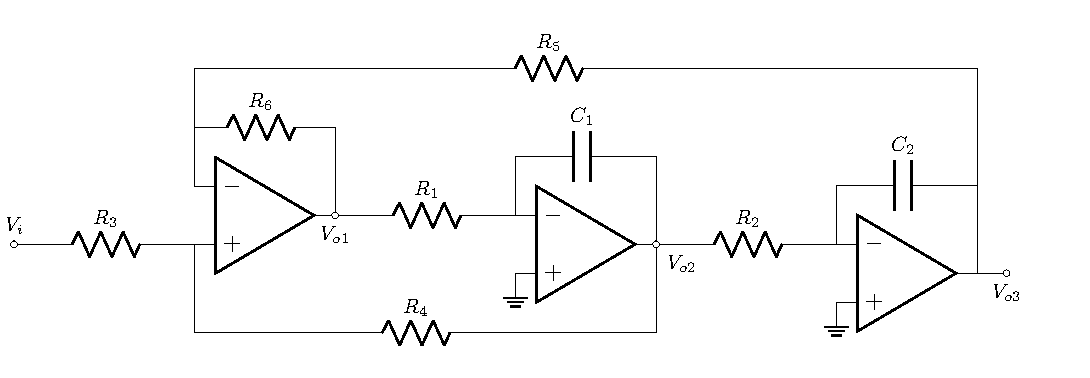
\includegraphics[width=0.9\textwidth]{ImagenesEjercicio4/KHN.pdf}
	\caption{Celda KHN.}
	\label{fig:KHN}
\end{figure}

Con todo lo establecido previamente se consigue determinar las siguientes transferencias:
\begin{equation}
	\frac{V_{o3}}{V_{o1}} = \frac{R_5 + R_6}{R_4 + R_3} \frac{R_3}{R_5} \frac{1}{D(s)}
	\label{equ:pbajo}
\end{equation}

\begin{equation}
	\frac{V_{o2}}{V_{o1}} = -\frac{R_5 + R_6}{R_4 + R_3} \frac{R_3}{R_5} \frac{s}{R_1 C_1 D(s)}
	\label{equ:pband}
\end{equation}

\begin{equation}
	\frac{V_{o2}}{V_{o1}} = \frac{R_5 + R_6}{R_4 + R_3} \frac{R_3}{R_5} \frac{s^2}{D(s)}
	\label{equ:palto}
\end{equation}

Siendo
\begin{equation*}
	D(s) = S^2 + \frac{s}{R_1 C_1} \frac{R_5 + R_6}{R_4 + R_3} \frac{R_3}{R_5} + \frac{R_6}{R_1 R_2 R_5 C_1 C_2}
\end{equation*}

Observando (\ref{equ:pbajo}), (\ref{equ:pband}) y (\ref{equ:palto}), se denota tomando cada una de dichas salidas, esta celda puede ser utilizada como un pasa bajos, pasa banda y pasa altos respectivamente. Tanto la frecuencia de corte, como el factor Q de cada etapa, es el mismo, ya que comparten denominador, siendo estos

\begin{equation}
\begin{split}
	\omega_o = \sqrt{\frac{R_6}{R_1 R_2 R_5 C_1 C_2}} \\
	Q = \frac{R_3 + R_4}{R_5 + R_6} \frac{R_5}{R_4} \sqrt{\frac{R_1 R_5 C_1}{R_2 R_5 C_2}} 
\end{split}
\end{equation}

Además, se destaca que la etapa que cumple el rol de pasa banda es inversora, detalle que no se cumple para el pasa bajos y altos. Por otro lado, en caso de ser deseado que esta celda funcione como un rechaza banda, se debe agregar un cuarto amplificador operacional que actúe como restador de las tres señales previamente mencionadas.
\begin{figure}[H]
\begin{center}
\begin{circuitikz}
	\node [circ](central){};
	\draw (central) -- ++(0,1) to[R, l=$R_{PB}$] ++(-2,0) node[ocirc, label=left:$V_{o3}$](){};
	\draw (central) to[R, l=$R_{PBanda}$] ++(-2,0) node[ocirc, label=left:$V_{o2}$](){};
	\draw (central) -- ++(0,-1) to[R, l=$R_{PA}$] ++(-2,0) node[ocirc, label=left:$V_{o1}$](){};
	\draw (central) -- ++(1,0) node[op amp, anchor=-](Amp){};
	\draw (Amp.+) node[ground](){};
	\draw (Amp.-) -- ++(0,1) to[R, l=$R_f$] ++(2.25,0) -| (Amp.out);
	\draw (Amp.out) -- ++(0.5,0) node[ocirc, label=right:$V_{RB}$](){};
\end{circuitikz}
	\caption{Configuración restadora para obtener un rechaza banda con filtro KHN.}
	\label{fig:khninv}
\end{center}
\end{figure}

\subsubsection{Tow-Thomas}

\subsubsection{Ackerberg-Mossberg}

\subsubsection{Fleischer-Tow}

\end{document}
